74. $\cfrac{x\sqrt{x}+x-5\sqrt{x}+2}{\sqrt{x}-2}\geqslant x \Leftrightarrow \begin{cases} t=\sqrt{x}\geqslant0,\\ \cfrac{t^3+t^2-5t+2}{t-2}\geqslant t^2.\end{cases}
\Leftrightarrow \begin{cases} t=\sqrt{x}\geqslant0,\\ \cfrac{t^3+t^2-5t+2}{t-2}\geqslant t^2.\end{cases}
\Leftrightarrow$\\$ \begin{cases} t=\sqrt{x}\geqslant0,\\ \cfrac{t^3+t^2-5t+2-t^3+2t^2}{t-2}\geqslant 0.\end{cases}
\Leftrightarrow \begin{cases} t=\sqrt{x}\geqslant0,\\ \cfrac{3t^2-5t+2}{t-2}\geqslant 0.\end{cases}
\Leftrightarrow \begin{cases} t=\sqrt{x}\geqslant0,\\ \cfrac{(t-1)(3t-2)}{t-2}\geqslant 0.\end{cases}$ Применив метод интервалов, найдём ответ: $t\in\left[\cfrac{2}{3};1\right]\cup(2;+\infty)\Leftrightarrow x \in\left[\cfrac{4}{9};1\right]\cup(4;+\infty).$
\begin{figure}[ht!]
\center{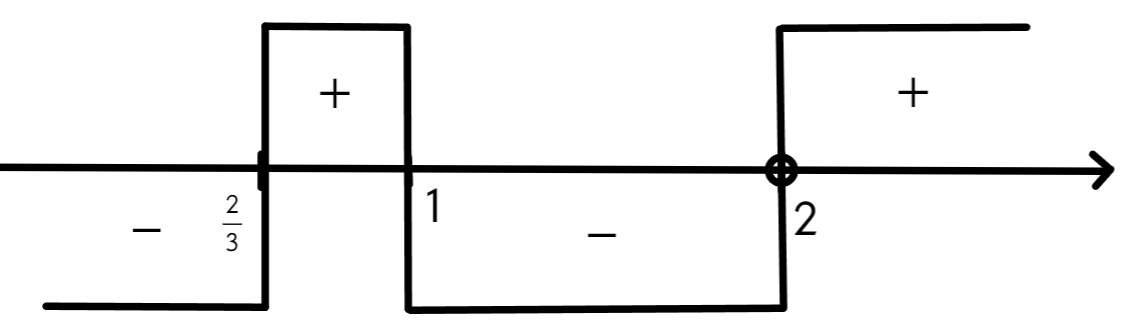
\includegraphics[scale=0.35]{int9-74.png}}
\end{figure}\\
